\documentclass{article}
\usepackage[utf8]{inputenc}
\usepackage{indentfirst}
\setlength{\parindent}{2em}
\usepackage{CJK}
\usepackage[utf8]{inputenc}
\usepackage{natbib}
\usepackage{graphicx}
\begin{document}
\begin{CJK}{UTF8}{gbsn}
\title{没想好名字}
\author{郑兴毫 朱解语 
      \\(各占百分之五十)}
\date{}
\maketitle
\renewcommand{\contentsname}{目录}
\tableofcontents
\section{摘要}

\label{sec:introduction}
\section{股权激励}
《史记·范雎蔡泽列传》中有“内务两江,而外多敌国,吾是以忧……欲以激励”之说,由是可见激励制度古已有之。最早提出“激励”概念的是中国学者,而今这一方法东西方已被广泛应用于现代企业的运营管理中。作为激励制度的一部分,股权激励有如下两种典型方式:其一为员工持股计划(Employee Stock Ownership plan,简称ESOP),以企业内部普通员工为对象,指由员工出资认购其所在公司股权,并将所购股权委托给员工持股平台,最终通过该平台实现股息分享和股权变现的一种新型股权模式;其二为管理层股票期权(Executive Stock Options,简称ESO),以企业高层管理人员及部分特殊员工为对象,指企业在未来一定期限内有条地件授予上述二者以预先约定价格购买本公司股票权利的激励形式。二者虽有不同,本质上都是为了通过激励手段增强员工积极性,从而建立提升企业效益的相对长久的机制。\\

有学者认为股权激励滥觞于二十世纪五六十年代的美国,实则不然。股权作为激励方式起始于中国,山西晋商曾建立完善的“身股”制度,“东家”和“掌柜”的关系,类同于现在“股东”和“经理”的关系,有效地分离了资本的所有权和经营权,在明末清初广为盛行.\\

但在今天,“美国7000家以上上市公司中90\%以上都做了股权激励,美国的高科技企业基本100\%都做了股权激励。而中国的情况,据我们前一段时间的统计,只有30\%的上市公司做了股权激励。”不过就未来趋势而言,中国选择股权激励的企业数量势必会不断攀升。本文将以美国谷歌公司为例,着重分析其采用的股权激励方式及产生的影响,并取其精华,为我国企业思考借鉴之处,从而结合国情和具体企业情况探索出适合我国现代企业的股权激励道路。
\section{谷歌公司简介}

\subsection{公司现状}
Google是一家大型跨国科技公司,它于1998年成立为一家私营公司,并于2004年8月19日开始公开交易,专门从事与互联网相关的服务和产品,其中包括在线广告技术,搜索引擎,云计算,软件和硬件。在2015年8月,Google进行宣布资产重组,重组后,Google被划归到新成立的Alphabet底下。\\Google这家超级大公司重组后,内部上下整体构架和运营构架皆实现了巨大的调整和改变:Alphabet成为多家公司的联合体,谷歌是其下最大的公司;创始人和原CEO拉里•佩奇(Larry Page)以及谷歌联合创始人谢尔盖•布林(Sergey Brin)将继续担任新公司Alphabet的高层领导。佩奇会担任Alphabet公司的CEO,布林为新公司总裁,从摩根士丹利跳槽谷歌担任财务长的Ruth Porat将出任Alphabet和谷歌的财务长。\\从近几年发展战略来看,Google从Mobile First调整为AI First, Google Assistant使用范围不断扩大,2017年10 月的秋季发布会上,Google发布了Pixel 2、Pixel 2 XL,全新的智能音箱Google Home Mini、Google Home Max以及全新的笔记本Google Pixelbook 等多款重量级硬件产品。Google正在向人工智能方向迅速发展,前景十分可观。

\subsection{谷歌的激励体系}
\subsubsection{基于绩效考核的奖励}
奖励(除期权和股票增值权(SARs)以外)是基于员工业绩来授予的,与以下一项或多项绩效指标相关:\\
资本存量的市场价格,股本收益,收入,净收入或利润(税前或税后),经济利润,营业收入,营业利润率,利润率,毛利率,股东权益或股东权益,股东总回报,市值,企业价值,现金流量(包括但不限于经营现金流量和自由现金流量),资金头寸,资产或净资产收益率,资本回报率,投资资本回报率,销售回报率,股东回报率,经济附加值,现金增值,收益或净收益(利息,税收,折旧和摊销前后),持续经营收益,营业收入,可控利润,销售或收入,销售增长,新订单,资本或投资,债务与债务加权益比率,营业收入与资本支出的比率,产品创新,产品发布时间表与市场目标,市场份额,成本削减目标,库存或供应链管理计划,预算比较,指定项目或流程的实施或完成,客户满意度MBO(目标管理),生产力,费用,利润率,运营效率,营运资金,合资企业的形成,研发合作,或完成其他交易。(可根据GAAP确定的任何其他财务业绩衡量标准,或前述任何组合。)
\subsubsection{基于GSU和期权的股权激励}
\section{谷歌股权激励计划}
\subsection{简介}
正如2012年Google雇员奖金激励计划的报告里所指出的,“本计划旨在通过向员工和顾问提供奖励来促进公司及其股东的利益,以鼓励他们继续为公司服务,提高公司的盈利能力和使公司实现财务上的成功。”Google,和其他任何公司一样,都是
Google的股权激励主要是通过期权和GSU(Google Stock Unite)实现的,在一定的等待期后(大部分新员工需要等待一年左右),1股GSU便可以转化为谷歌的股票,
\subsection{期权}
首先,Google对发放给员工的期权做了很强的限制:“期权不得以任何方式出售,质押,转让,或以任何其他方式处置,也不能通过遗嘱或递延法律或分配法律”。\\
其次,关于期权的行使价格,在Google上市前后有一些变化,在Google上市之前,它将期权行使价格设定为其市场价值的内部估计值。从谷歌创始到2003年初,这个估计值是不变的,2003年开始,它每个月大约上调一次(Bo and Eric, 2015)。
图1是从2003年开始到第一次IPO的\\
 \begin{figure}
  \centering
  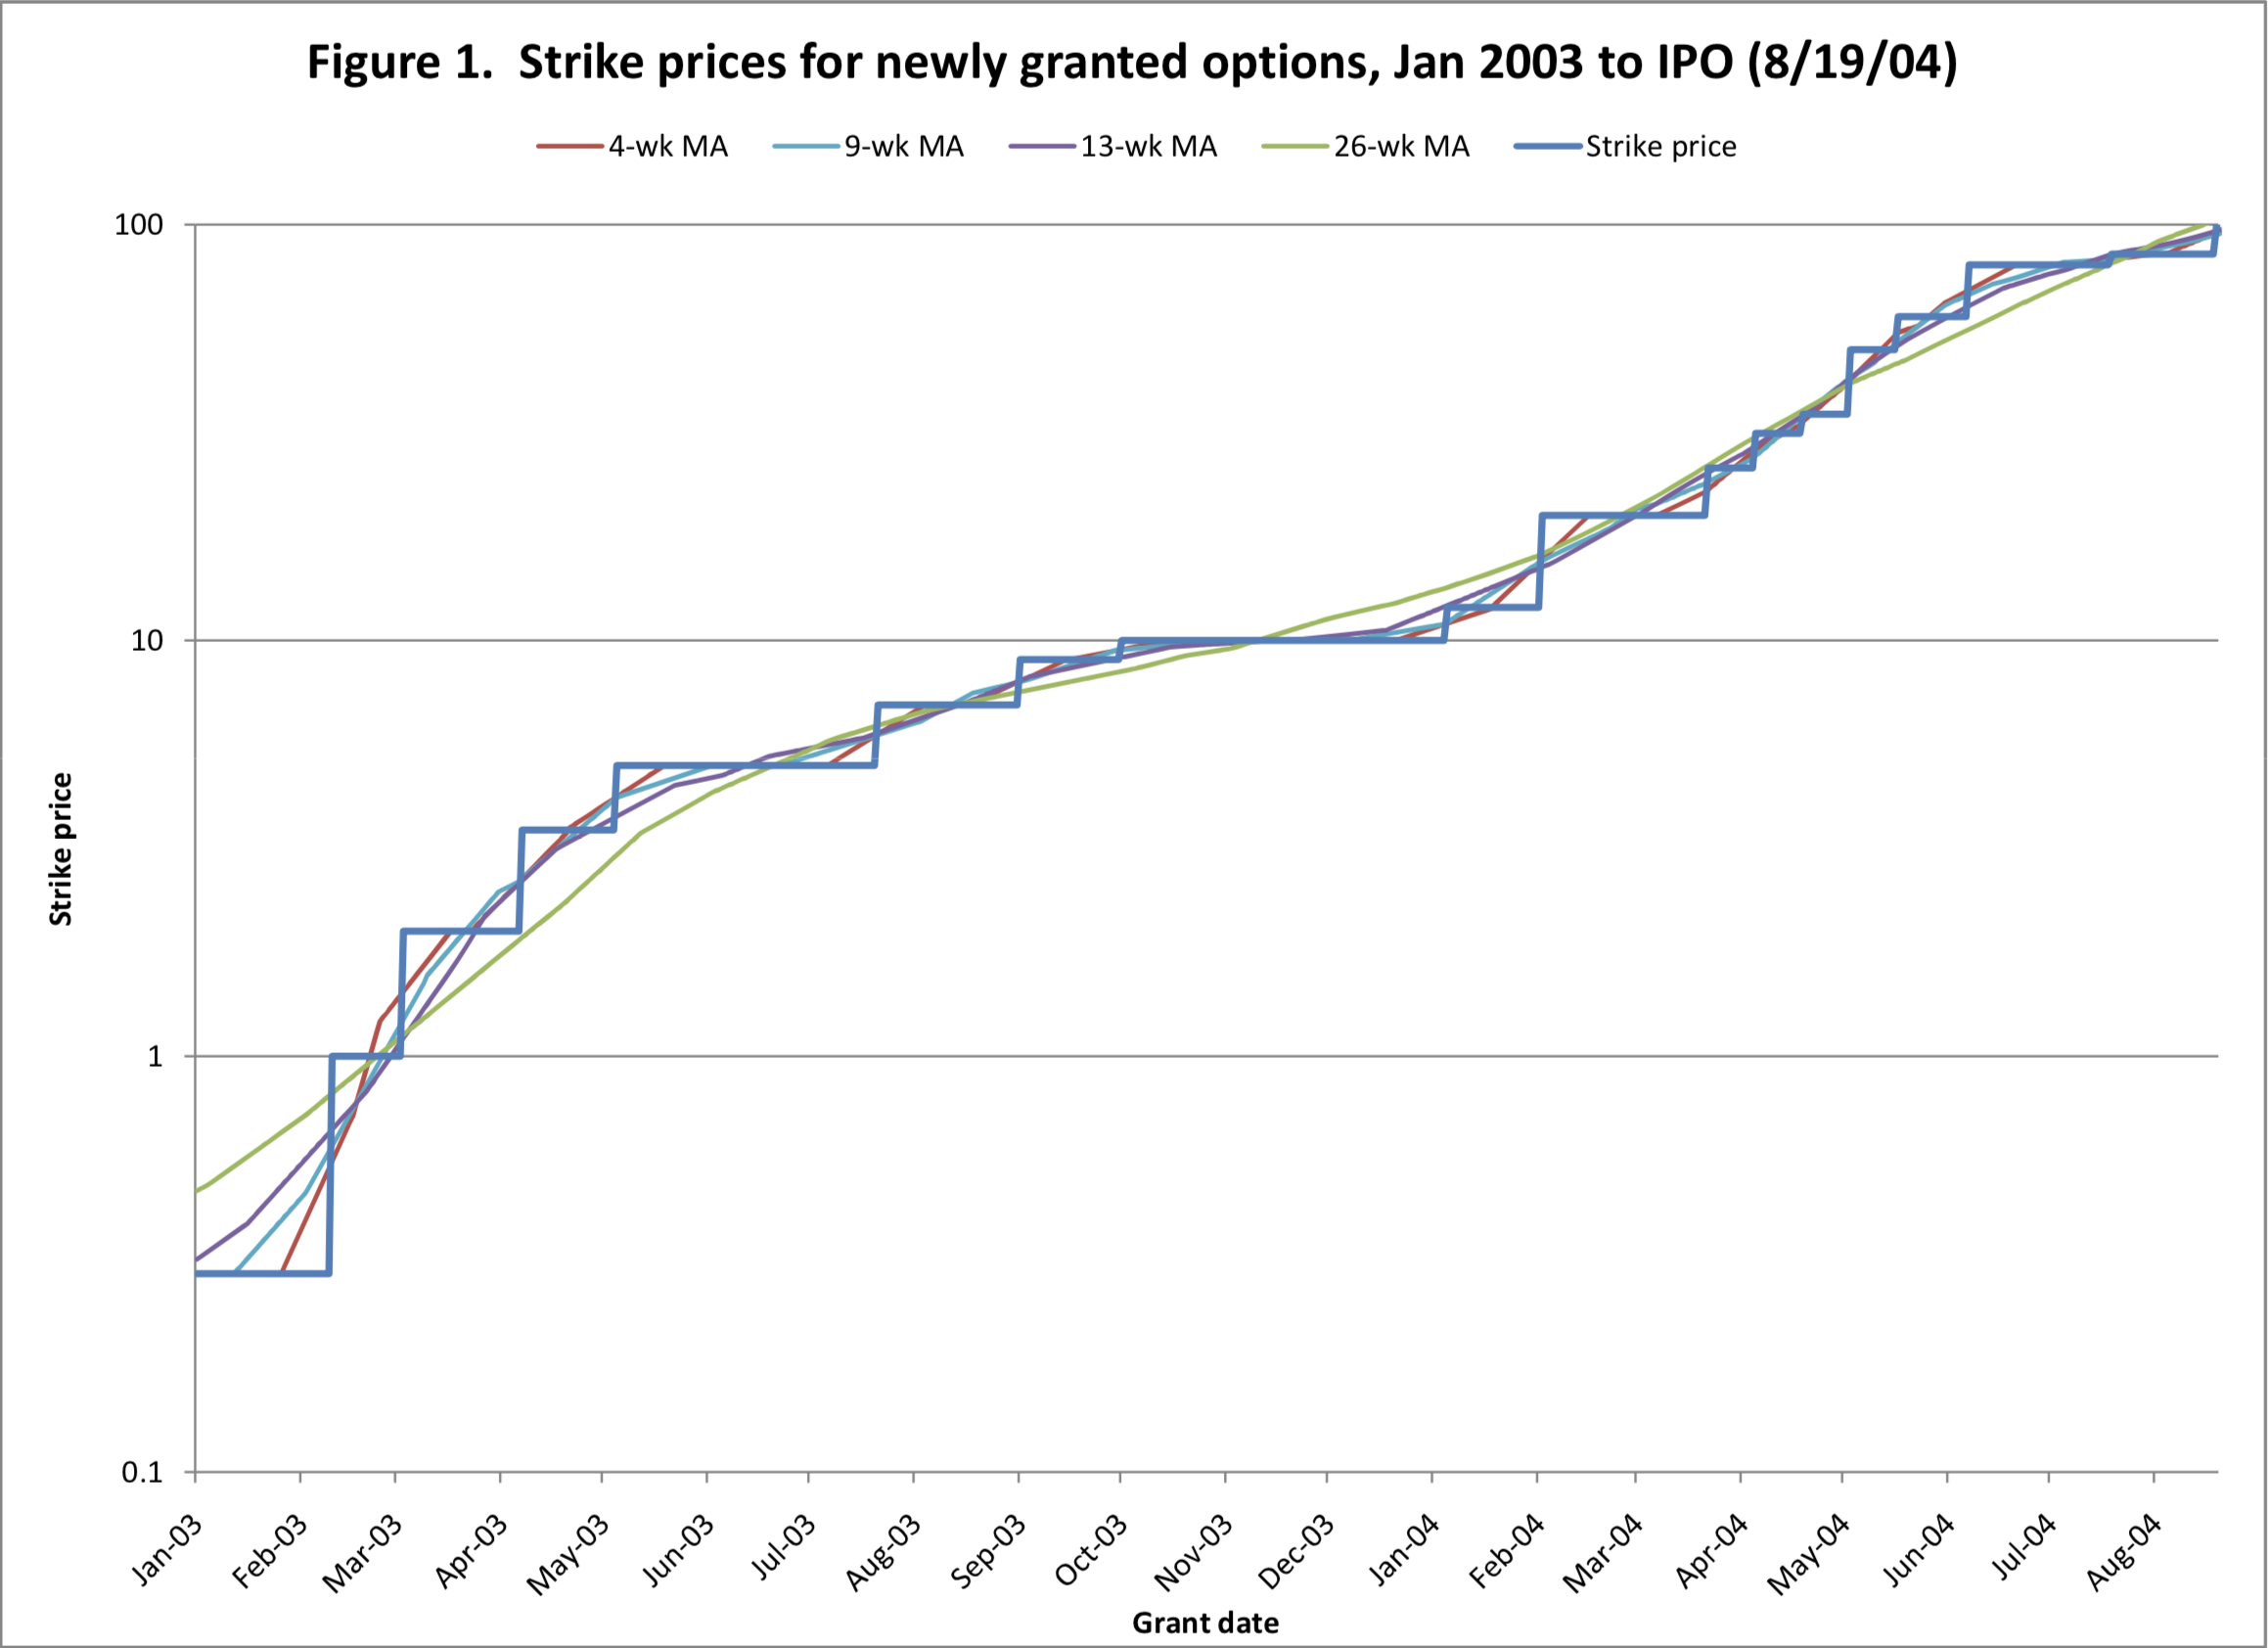
\includegraphics[width=1\textwidth]{1.png} 
  \caption{Strike prices for newly granted options} 
  \label{img}
 \\
\subsection{GSU}
\end{figure}
\end{CJK}


\end{document}
